\section{What we find}\label{sec:structure}

What do the groups look like on the archive, and what holds them together? The groups are those
labelled by the method of the note \emph{Group flights in free flight}, with its chosen values,
$\delta=2$~min and $q=0.1$: 21.7\% of the paraglider flights and 6.9\% of the hang-glider
flights fly in a group at some point, in 17\,169 episodes (Table~\ref{gi-tab:q} of the note).
Chance is the null model of Section~\ref{gi-sec:null} of the note; bands are 5--95\% of 200 draws
of the dependency blocks, or of the dates where the captions say so. Graph terms are defined in
Appendix~\ref{app:graphs}, the two models in Appendix~\ref{app:models}. The report
\emph{Group and solo flights} (\texttt{analysis/groups/group-identification}) compares the motion
of pilots in a group and alone; some results here refer to it.

\subsection{What the groups are}\label{sec:sizes}

How large are the groups, how long do they last, and how do they change? We count episodes and
groups (Section~\ref{gi-sec:groups} of the note) by number and by duration; an episode lasts from the start of
its first group to the end of its last, and its participants are the distinct flights it holds.

\begin{figure}
\centering
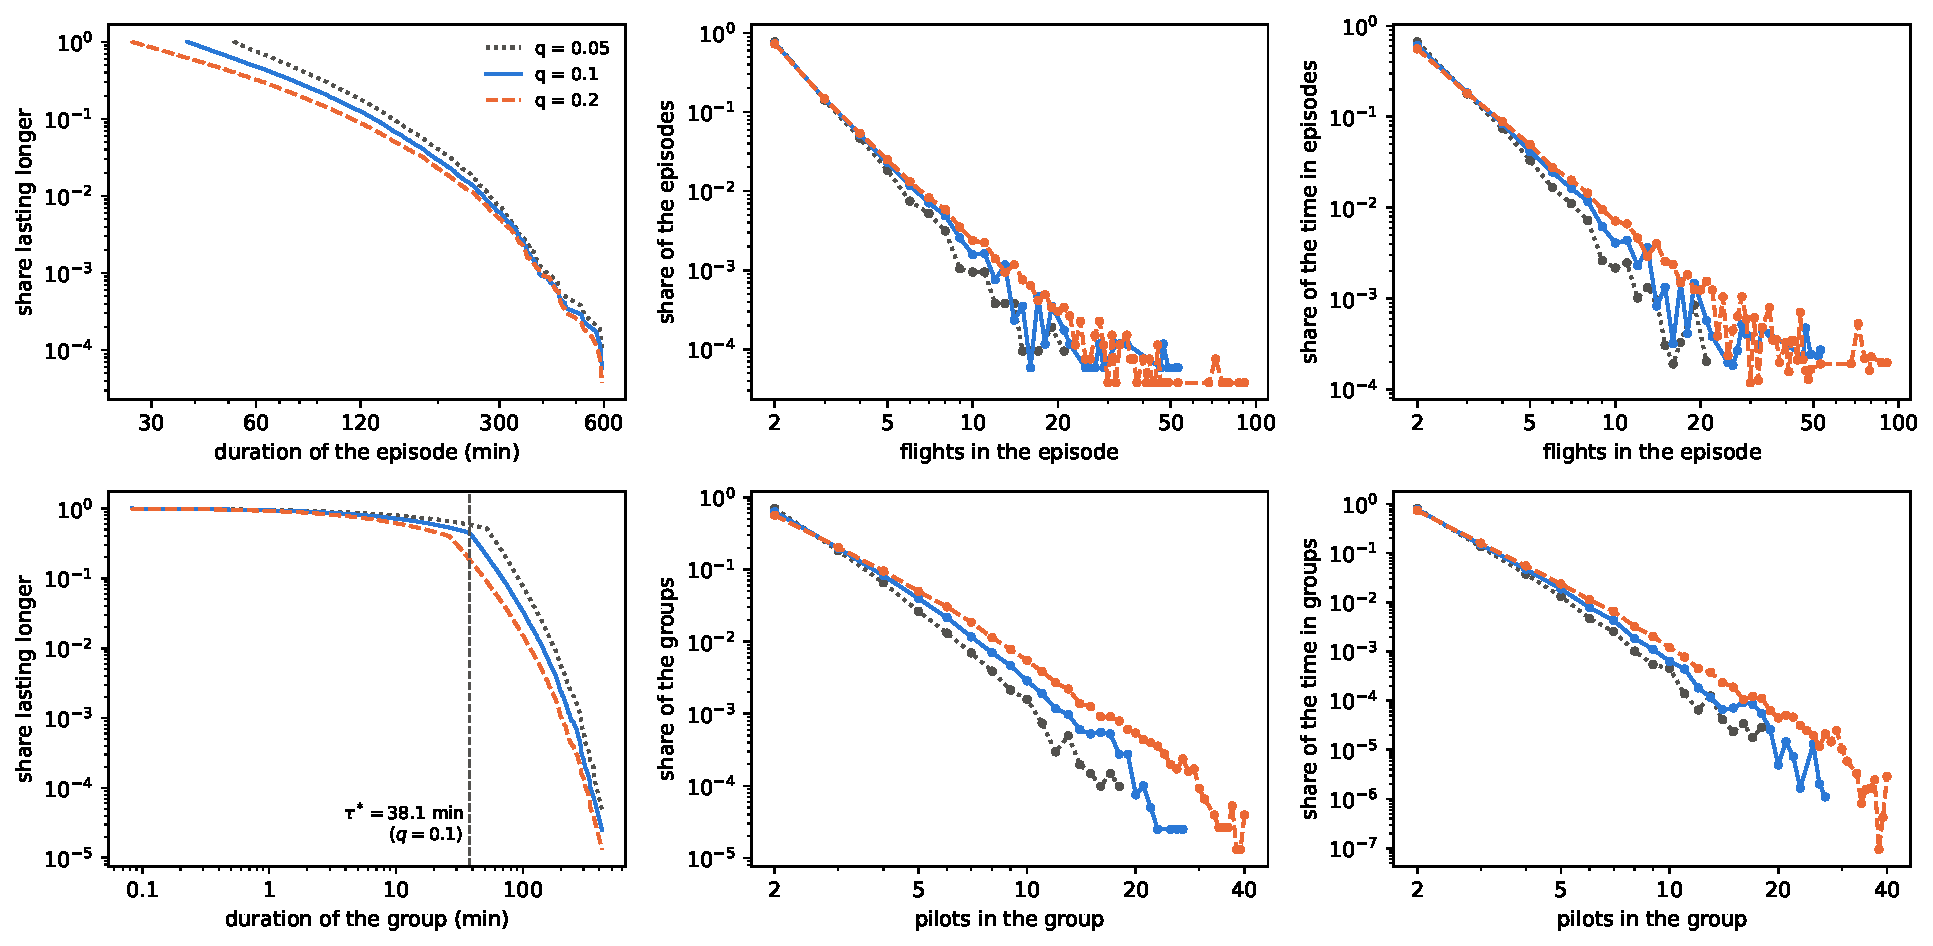
\includegraphics[width=\textwidth]{../../../methods/group-identification/figures/assessment_structure.pdf}
\caption{Episodes (top) and groups (bottom), $\delta=2$~min, whole archive, for three
values of $q$. Left: share lasting longer than a duration. Middle: share of each size. Right:
share of the total duration in each size.}
\label{fig:structure}
\end{figure}

\begin{table}
\centering
\small
\begin{tabular}{@{}l l r r c c c c r@{}}
\toprule
& $q$ & number & median & \multicolumn{2}{c}{2 participants} & \multicolumn{2}{c}{5 or more} & largest \\
& & & duration & items & time & items & time & \\
\midrule
episodes & 0.05 & 10\,553 & 74.6 min & 77\% & 67\% & 3.9\% & 8.1\% & 21 \\
 & 0.1 & 17\,169 & 58.2 min & 74\% & 61\% & 5.7\% & 12.6\% & 53 \\
 & 0.2 & 26\,504 & 44.5 min & 73\% & 56\% & 7.0\% & 17.2\% & 91 \\
\midrule
groups & 0.05 & 20\,275 & 52.7 min & 70\% & 81\% & 5.6\% & 2.3\% & 18 \\
 & 0.1 & 40\,051 & 30.4 min & 63\% & 77\% & 9.4\% & 3.5\% & 27 \\
 & 0.2 & 75\,953 & 17.1 min & 56\% & 74\% & 14.1\% & 5.0\% & 40 \\
\bottomrule
\end{tabular}
\caption{Episodes and groups for three values of $q$ ($\delta=2$~min). Items: share of the
episodes or groups of that size; time: share of their total duration.}
\label{tab:structure}
\end{table}

\paragraph{Sizes and durations.} With the chosen values the median episode lasts 58.2~min and three
in four are pairs (Table~\ref{tab:structure}). Episodes last at least $\tau^*$, since a contact
must, and larger episodes last longer, so they weigh more in time than in number. Groups have no
minimum duration: every arrival or departure of a member starts a new one, so 10\% last less
than 2.1~min, and the median is 30.4~min. Large groups change quickly, so in time the pairs weigh
more than in number. \StWithHang\% of the groups hold a hang glider. Inside a group the edges
among the members can change: the 40\,051 groups of the chosen values hold 52\,856
configurations. A larger $q$, hence a shorter $\tau^*$, gives more, shorter and larger groups:
the shares of the small sizes change little, and the tail moves.

\paragraph{How groups change.}\label{sec:describe} A group ends in one of five ways: a
\emph{join} (members added), a \emph{leave} (members removed in flight), a \emph{landing} (a
removed member lands within 5~s, the grid step), a \emph{split} or a \emph{merge}
(Appendix~\ref{app:graphs}); a group of two pilots that loses one dissolves.
Table~\ref{tab:rates} gives, by size, the groups ending per hour spent at that size.
\begin{itemize}
  \item \textbf{Most episodes never change:} \StEpisodeSingle\% of the \StEpisodes{} episodes are one
        group; \StEpisodeSplit\% hold a split, \StEpisodeMerge\% a merge.
  \item \textbf{Episodes last; groups change.} \StEpisodeTwoHours\% of the episodes last 2~h or
        more. A group lasts \StMedianGroupTwo~min with 2 pilots and \StMedianGroupMax~min with
        \StSizeMax{} or more: joins, leaves, splits and merges all grow with size, so a large group
        changes members every few minutes.
  \item \textbf{Groups break in flight:} \StEndFlight\% of the \StEnds{} groups that dissolve do
        so in flight, \StEndLanding\% at a landing; a pair ends mostly because the two separate.
        \StFormDeparture\% of the \StFormations{} groups with no predecessor form when a member
        departs: pilots who took off together.
\end{itemize}

\begin{table}
\centering
\footnotesize
\begin{tabular}{@{}r r r l l l l l@{}}
\toprule
pilots & hours & median (min) & join & leave & landing & split & merge \\
\midrule
2 & 17\,389 & 41 & 0.31\,{\tiny[0.30, 0.32]} & 0.96\,{\tiny[0.95, 0.97]} & 0.098\,{\tiny[0.094, 0.10]} & -- & 0.085\,{\tiny[0.079, 0.092]} \\
3 & 3\,349 & 20 & 0.54\,{\tiny[0.52, 0.57]} & 1.6\,{\tiny[1.6, 1.6]} & 0.050\,{\tiny[0.044, 0.056]} & -- & 0.16\,{\tiny[0.15, 0.18]} \\
4 & 1\,059 & 13 & 0.70\,{\tiny[0.66, 0.76]} & 1.6\,{\tiny[1.6, 1.7]} & 0.042\,{\tiny[0.032, 0.051]} & 0.48\,{\tiny[0.45, 0.52]} & 0.26\,{\tiny[0.22, 0.29]} \\
5 & 421 & 11 & 0.88\,{\tiny[0.80, 0.96]} & 1.7\,{\tiny[1.6, 1.8]} & 0.036\,{\tiny[0.021, 0.057]} & 0.82\,{\tiny[0.76, 0.88]} & 0.32\,{\tiny[0.26, 0.37]} \\
6 & 176 & 8 & 1.1\,{\tiny[0.93, 1.2]} & 2.1\,{\tiny[1.9, 2.3]} & 0.028\,{\tiny[0.011, 0.048]} & 1.2\,{\tiny[1.0, 1.3]} & 0.51\,{\tiny[0.40, 0.63]} \\
7 & 96 & 7 & 1.1\,{\tiny[0.91, 1.3]} & 2.0\,{\tiny[1.8, 2.2]} & 0.031\,{\tiny[0.0089, 0.074]} & 1.3\,{\tiny[1.1, 1.5]} & 0.40\,{\tiny[0.30, 0.53]} \\
8+ & 107 & 4 & 1.8\,{\tiny[1.5, 2.2]} & 2.5\,{\tiny[2.2, 2.8]} & 0.028\,{\tiny[0.0084, 0.057]} & 2.7\,{\tiny[2.4, 3.1]} & 1.0\,{\tiny[0.73, 1.2]} \\
\bottomrule
\end{tabular}

\caption{By size: hours spent, median duration of a group, and groups ending per hour by
outcome, with 5--95\% bands.}
\label{tab:rates}
\end{table}

\paragraph{Where in the flight.}\label{sec:phases} On 1~Hz flights, where the phases are labelled,
we take the phase at the instant a flight enters (\Entries{}) or leaves (\Exits{}) a group; entries
at the departure (\AtDeparture{}) and exits at the landing (\AtLanding{}) are counted apart. Both
follow the shares of the time alone in each phase (Table~\ref{tab:phases} in
Appendix~\ref{app:evidence}): there is no phase where groups preferentially form or break.
\EntriesEarly\% of the entries are within 10~min of the departure.

\paragraph{When in the day.}\label{sec:hours} Group time is concentrated around midday:
\GroupShareNoon\% of a group flight's time at \GroupShareNoonHour~h, \GroupShareMorning\% at 9~h,
\GroupShareEvening\% at 18~h (Figure~\ref{fig:hours} in Appendix~\ref{app:evidence}).

\subsection{What keeps two pilots together}\label{sec:group-structure}\label{sec:cohesion}

Do two pilots in a group keep the same pace, or are they pulled back to each other? We follow the
delay $\ell^*(t)$ inside each contact (Appendix~\ref{gi-sec:lag} of the note), leaving out the instants with either
pilot in a search. Groups are the \StCohReal{} pair intervals of pilots who took off within 10~km;
chance is the \StCohChance{} contacts of the surrogate pairs, two pilots who never saw each other,
and the \StCohChanceLong{} of these that last at least $\tau^*$, selected as the groups are. Three
measures:
\begin{itemize}
  \item $D(s)=\langle(\ell(t+s)-\ell(t))^2\rangle$, the mean square change of the delay after $s$,
        fitted by an Ornstein--Uhlenbeck process, $D(s)=2\sigma^2(1-e^{-ks})+c$: $1/k$ is how long
        the delay remembers its value, $\sigma$ its spread, $2k\sigma^2$ how fast it wanders;
  \item the drift $\langle\ell(t+60~\mathrm{s})-\ell(t)\rangle/60~\mathrm{s}$ at each $\ell$, made
        symmetric since the order of a pair is arbitrary: the pull back to $\ell=0$, a spring $-k\ell$
        near 0;
  \item the distance between the two pilots at the same instant after their first contact. Two
        independent pilots separate as twice the displacement variance of one, since the drift along
        the route cancels in their difference; the surrogate pairs give this baseline on the same
        terrain.
\end{itemize}

\begin{figure}
\centering
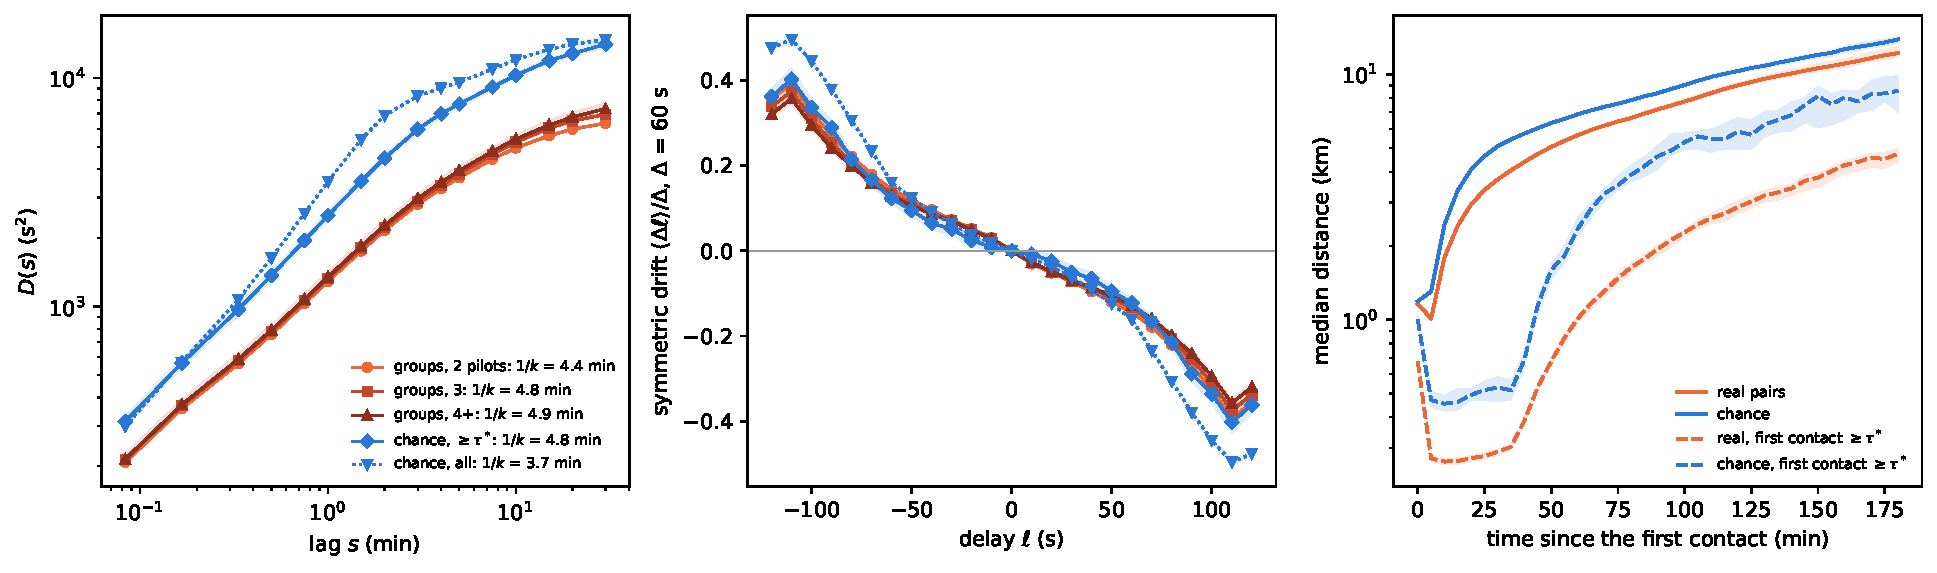
\includegraphics[width=\textwidth]{figures/structure/cohesion.pdf}
\caption{Left: $D(s)$ of groups (by size) and of chance contacts, with $1/k$ of the
Ornstein--Uhlenbeck fit. Middle: symmetric drift of the delay. Right: median distance at the same
instant after the first contact, for every pair and for those whose first contact lasts at least
$\tau^*$. Bands: 5--95\% of 200 draws of the dates.}
\label{fig:cohesion}
\end{figure}

\begin{itemize}
  \item \textbf{Groups keep the same pace.} Their delay wanders at $2k\sigma^2=\StQReal$ \StQRealBand~s$^2$/s,
        against \StQChanceLong{} \StQChanceLongBand{} for chance contacts as long and \StQChance{}
        \StQChanceBand{} for all of them; its spread is $\sigma=\StSigmaReal$~s \StSigmaRealBand, against
        \StSigmaChance~s \StSigmaChanceBand. Size does not matter: $2k\sigma^2=\StQTwo$, \StQThree{} and
        \StQFour~s$^2$/s at 2, 3 and 4+ pilots.
  \item \textbf{They are not pulled back much harder.} The delay forgets itself in $1/k=\StOuReal$~min
        \StOuRealBand, against \StOuChance~min \StOuChanceBand{} by chance; the drift gives \StDriftReal~min
        \StDriftRealBand{} against \StDriftChance~min \StDriftChanceBand. Most of the pull is the
        selection: a contact that lasts keeps $|\ell|\le\delta$ by definition.
  \item \textbf{They stay together after the contact that selected them.} When the first contact lasts
        at least $\tau^*$, the two pilots are \StSepRealLongSixty~km apart 60~min later (median), against
        \StSepChanceLongSixty~km by chance; \StSepRealLongTwoHours{} against \StSepChanceLongTwoHours~km
        after 2~h. Over every first contact, \StSepRealThirty{} against \StSepChanceThirty~km after 30~min.
\end{itemize}
What holds a group together is a shared pace; a spring adds little to it. Whether the shared pace
is following or the same choices in the same air, the data cannot tell.

\subsection{Who leads}\label{sec:leaders}

Who is ahead in a group, how often does that change, and who is it? The answer starts from the
shape of the group.

\paragraph{Shape.}\label{sec:chains} Inside a group the members are fixed, but the pair intervals
among them start and end: each edge set is a configuration. A configuration has a density, a
diameter and a shape: complete, a tree (a chain or a star), or between (Appendix~\ref{app:graphs}).
The TA-MSD pieces of the report \emph{Group and solo flights} lie inside one group and take the
shape of its configuration at their middle.
\begin{itemize}
  \item \textbf{Large groups are strings along the route.} Three pilots form a triangle \StTriangleThree\%
        of the time and a chain \StChainThree\%. Complete graphs fall from \StCompleteFour\% of the time
        at 4 pilots to \StCompleteMax\% at 8+, the mean density from \StDensityThree{} at 3 to
        \StDensityMax{} at 8+; at 8+ the diameter is 4 or more \StDiamFourMax\% of the time: pilots
        follow each other along the route.
  \item \textbf{The shape does not change the flight.} $H_\mathrm{loc}(1000~\mathrm{s})$ is
        \StHlocTriangle{} in triangles and \StHlocChain{} in chains; \StHlocComplete{} in complete graphs
        of 4+ and \StHlocTree{} in trees. The straighter progress found in \emph{Group and solo flights}
        does not need every pilot in contact with every other.
\end{itemize}

\begin{figure}
\centering
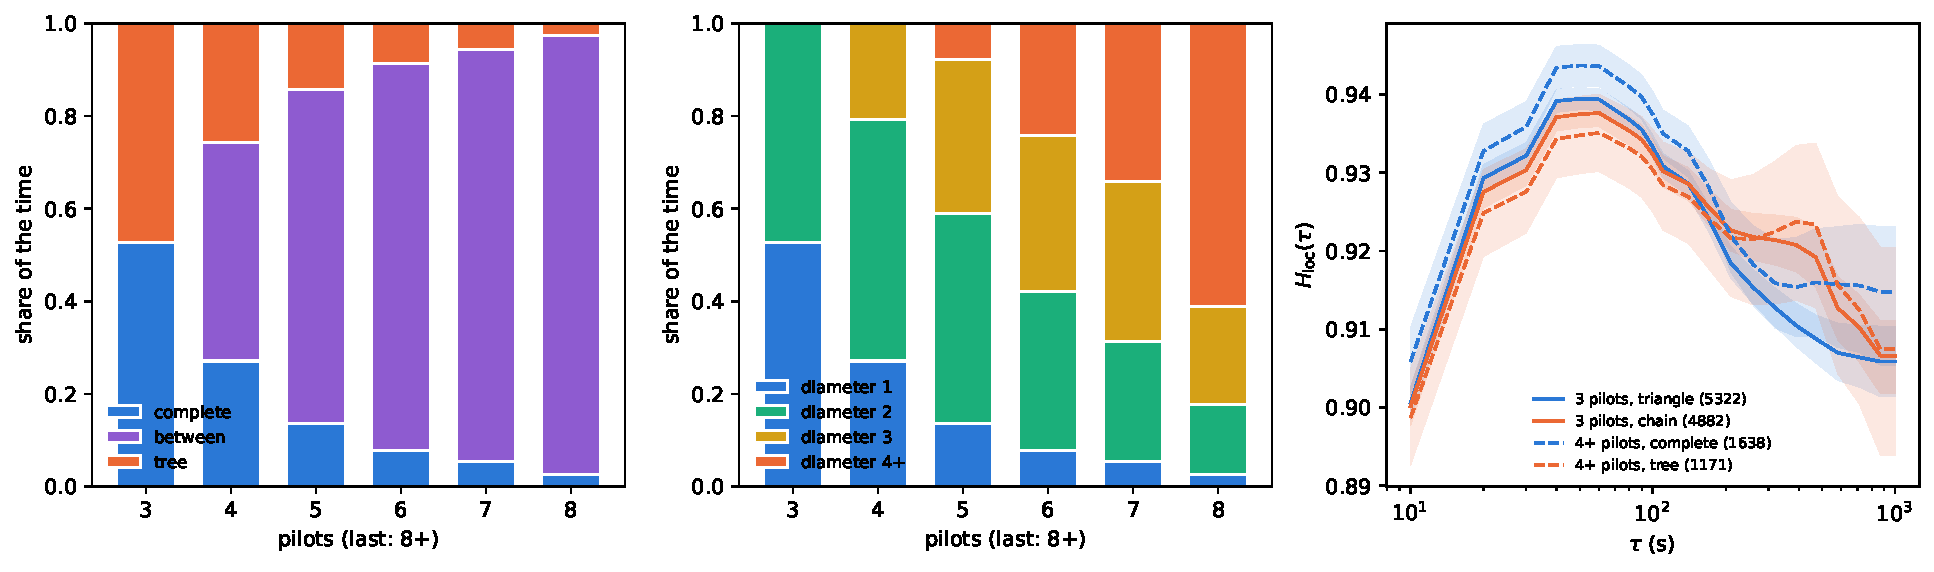
\includegraphics[width=\textwidth]{figures/structure/chains.pdf}
\caption{Left: share of the time of each shape, by size (8+ pooled). Middle: share of the time by
diameter. Right: $H_\mathrm{loc}(\tau)$ of paragliders in triangles and chains of 3 pilots, and in
complete and tree graphs of 4 or more (flights in brackets), with 5--95\% bands.}
\label{fig:chains}
\end{figure}

\paragraph{Order.} The signed median delay $\ell_{\rm med}$ of a pair interval
(Appendix~\ref{gi-sec:lag} of the note) says who passes first: the pilot ahead, when the other passes at least
15~s later; otherwise the two fly abreast (\Abreast\% of the pairs of two; median delay
\DelayMedian~s). How leading changes the flight is in \emph{Group and solo flights}; here we ask
who leads (Figure~\ref{fig:hierarchy}; Figure~\ref{fig:habitual} in Appendix~\ref{app:evidence}).
\begin{itemize}
  \item \textbf{Pilots are in a line.} In groups of 3 pilots or more, each edge points from
        the pilot ahead to the one behind; we compare with the same graphs with each direction drawn
        at random (50 draws). Directed triangles are cyclic \StCyclic\% \StCyclicBand{} of the time,
        against \StCyclicNull\% at random; graphs with every edge directed (\StFullShare\% of the time)
        are acyclic \StAcyclic\%, against \StAcyclicNull\%. Positions along one route cannot form
        cycles, so the order is geometry and says nothing about rank.
  \item \textbf{One leader, in small groups:} \StOneLeader\% \StOneLeaderBand{} of the acyclic time,
        against \StOneLeaderNull\% \StOneLeaderNullBand{} at random; \StOneLeaderThree\% at 3 pilots,
        \StOneLeaderFour\% at 4, \StOneLeaderFive\% at 5 or more. A single file (depth $n-1$):
        \StLineThree, \StLineFour{} and \StLineFive\%.
  \item \textbf{The lead changes often.} Along $\ell^*(t)$, with stretches shorter than 60~s dropped,
        the pilot ahead changes \StSwitches{} times per hour of contact \StSwitchesBand{}, against
        \StSwitchesChance{} \StSwitchesChanceBand{} in chance contacts lasting at least $\tau^*$; the
        pilot most often ahead holds \StDominant\% of the directed time (median), against
        \StDominantChance\%.
  \item \textbf{The experienced pilot on the faster wing leads.} In groups of two named
        pilots, the leader has more earlier flights in the catalog in \StExp\% \StExpBand{} of
        \StExpPairs{} pairs (\StExpRatio{} times as many, median), and the higher wing class (A~=~1 to
        competition~=~5) in \StWing\% \StWingBand{} of \StWingPairs.
  \item \textbf{Some pilots lead or follow persistently.} For the \HabitualPilots{} pilots with at
        least 10 roles in pairs, the dispersion of their lead fractions is \HabitualDispersion{}
        against \HabitualNull{} with roles swapped at random (95\% below \HabitualNullHigh);
        \HabitualExtreme\% lead in at most 20\% or at least 80\% of their roles, against
        \HabitualExtremeNull\% expected.
\end{itemize}

\begin{figure}
\centering
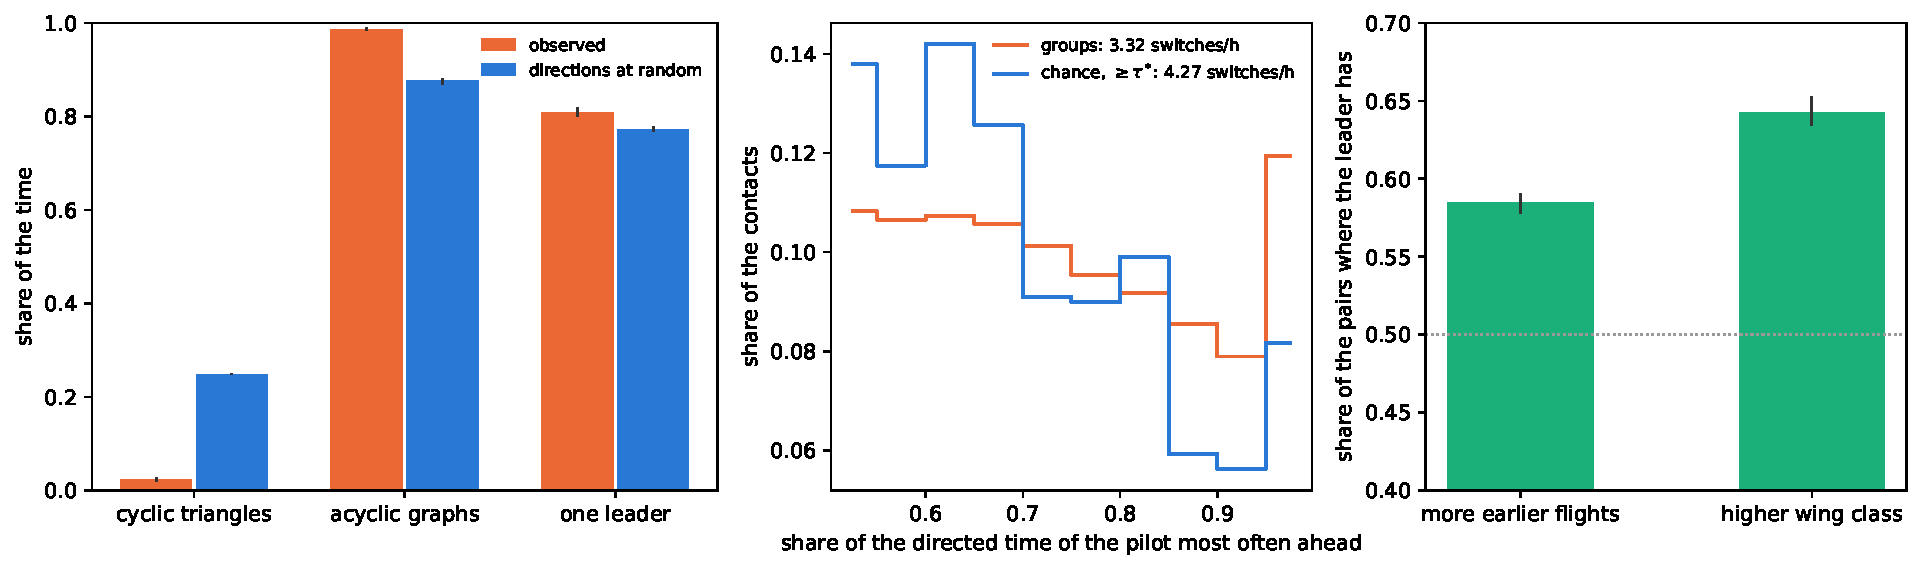
\includegraphics[width=\textwidth]{figures/structure/hierarchy.pdf}
\caption{Left: in groups of 3 or more, share of the time with cyclic directed triangles, acyclic
graphs (every edge directed) and one leader (acyclic graphs), observed and with directions at
random. Middle: share of the directed time of the pilot most often ahead in each contact, with the
switches per hour. Right: share of the pairs of two in which the leader has more earlier flights,
or the higher wing class. Bars: 5--95\% (blocks).}
\label{fig:hierarchy}
\end{figure}

\subsection{With whom}\label{sec:partners}

Do pilots choose their partners, or fly with whoever is there? We follow paraglider pilots by their
name in the catalog (anonymised ones left out). Two pilots are partners on a day when their
flights share a pair interval: a \emph{pair-day}. Chance keeps who flies in a group where and
when: within each site-day (takeoffs within 3~km, joined when a pair interval links two sites),
the partners are redrawn at random, each pilot keeping its number of partners that day (a
configuration model; 100 draws). There are \StPairDays{} pair-days among \StPilots{} pilots and
\StPairs{} pairs; one pair flew together on \StMaxDays{} days (Figure~\ref{fig:partners}).
\begin{itemize}
  \item \textbf{Pilots return to the same partners:} \StRepeatObs\% of the pair-days are on pairs
        that meet on more than one day, against \StRepeatNull\% \StRepeatNullBand{} at random
        (\StRepeatPairsObs{} such pairs against \StRepeatPairsNull).
  \item \textbf{and to their club:} \StSameClubObs\% of the pair-days join two pilots of the same
        club, against \StSameClubNull\% \StSameClubNullBand.
\end{itemize}
Chance already fixes who flies in a group at each site and day, so the excess is the choice of
partner among the pilots there. Choosing where and when to fly with friends stays in chance here.

\begin{figure}
\centering
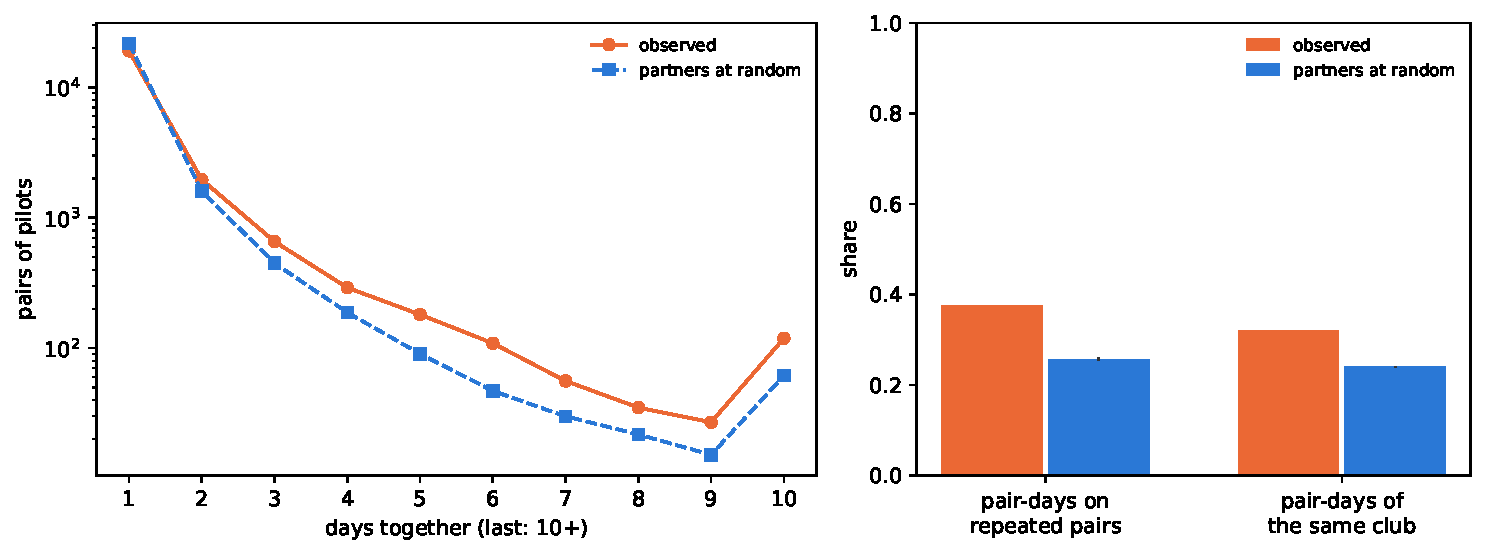
\includegraphics[width=0.85\textwidth]{figures/structure/partners.pdf}
\caption{Left: pairs of pilots by the number of days they flew together, observed and with
partners at random. Right: share of the pair-days on pairs that meet on more than one day, and of
two pilots of the same club (each pilot's main club); bars at random: 5--95\% of the draws.}
\label{fig:partners}
\end{figure}

\subsection{Where the sizes come from}\label{sec:fission}

Why are most groups pairs, and how do a few grow large? $T(n)$ is the share of the time spent in
groups of $n$ pilots: the chance that a group seen at a random instant has $n$ pilots. If
sizes change one pilot at a time, the flux from $n$ to $n+1$ pilots balances the flux back, a
birth--death chain (Appendix~\ref{app:models}):
\begin{equation}\label{eq:chain}
  \frac{T(n+1)}{T(n)}=\frac{g(n)}{l(n+1)},
\end{equation}
with $g(n)$ the joins and $l(n)$ the leaves and landings per hour at size $n$
(Table~\ref{tab:rates}); splits and merges are left out. Per member, $g(n)=a\,n$ and
$l(n)=\mu\,n^{1-\gamma}$: every member brings in others at rate $a$ and leaves at rate
$\mu n^{-\gamma}$. We fit these to the rates, without looking at $T$. With $\gamma=0$ the chain
gives the log-series $T(n)\propto x^n/n$, $x=a/\mu$. For comparison, we fit the form of Bonabeau
et al.~\cite{bonabeau1999}, $T(n)\propto n^{-\alpha}e^{-n/n_c}$, directly to $T$.

\begin{itemize}
  \item \textbf{One pilot at a time is enough.} With the measured rates the chain gives $T(n)$ within
        4\% from 2 to 8 pilots (\StChainThreePred{} against \StChainThreeObs{} at 3 pilots, just outside
        its band), although splits and merges are \StMultiTwo\% of the changes at 2 pilots and
        \StMultiMax\% at 8+.
  \item \textbf{Members join at a constant rate and leave less often in large groups.} Each member
        brings in others at $a=\StCapitaA$ \StCapitaABand{} per hour, at every size. Each leaves at
        \StLossTwo{} per hour in a pair and \StLossMax{} at 8+: $\gamma=\StGamma$ \StGammaBand.
  \item \textbf{The heavy tail comes from staying.} With $\gamma=0$ ($x=\StX$) $T(\StNTop)$ is
        \StLogSeriesFactor{} times too small; with $\gamma=\StGamma$, \StCapitaFactor{} times. Fitted
        directly, $\alpha=\StAlpha$ and $n_c=\StNc$.
\end{itemize}

\begin{figure}
\centering
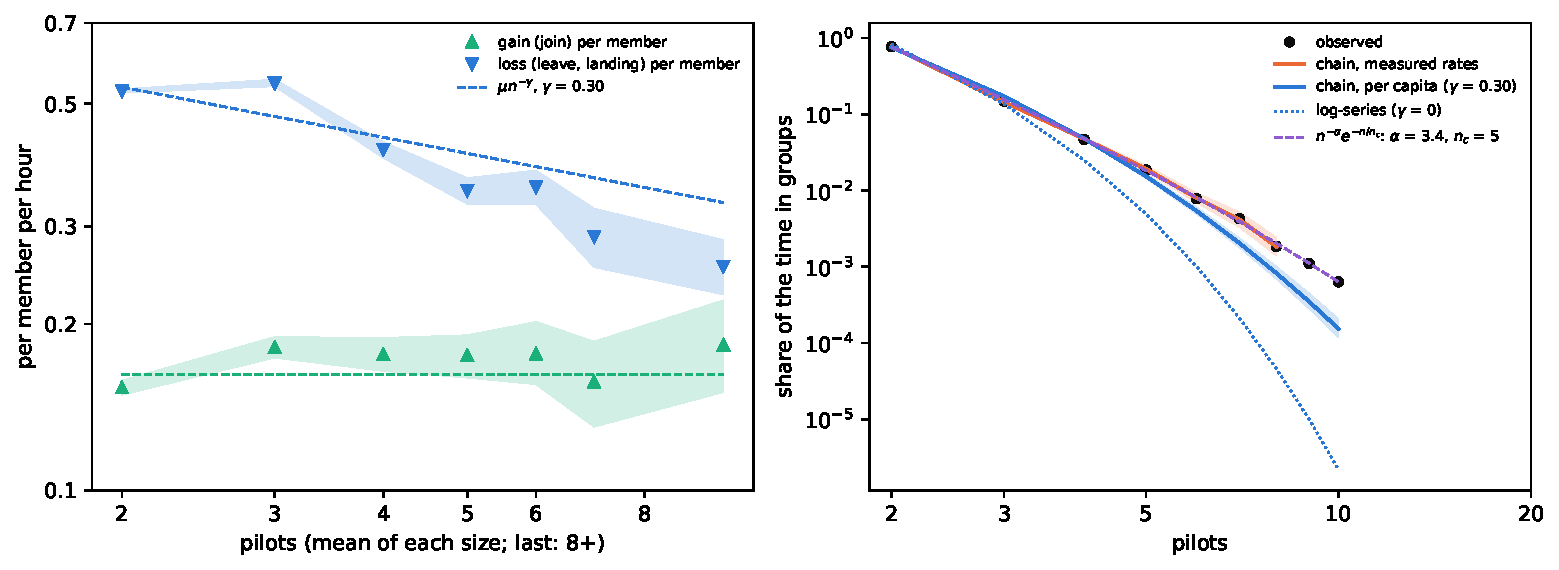
\includegraphics[width=0.9\textwidth]{figures/structure/fission.pdf}
\caption{Left: joins and losses per member per hour by size (mean size of each class; 8+ pooled),
with $a$ and $\mu n^{-\gamma}$ dashed. Right: $T(n)$ observed (sizes with at least 10~h) and from
the chain~\eqref{eq:chain} with the measured rates, with the per-capita rates and with $\gamma=0$;
dashed purple: the form of Bonabeau et al.\ fitted to $T$. Bands: 5--95\%.}
\label{fig:fission}
\end{figure}

\subsection{What the data support}\label{sec:conclusions}

\noindent
\begin{minipage}[t]{0.49\textwidth}
\textbf{Supported}
\begin{itemize}
  \item groups are mostly pairs; large ones are strings along the route that change members every
        few minutes, while the episode lasts about an hour;
  \item group pilots keep the same pace: their delay wanders half as fast as that of two pilots
        kept in contact by chance, and they stay closer after the contact;
  \item the size distribution follows from one pilot joining or leaving at a time; its heavy tail
        from members of larger groups leaving less often;
  \item the lead changes a few times per hour and goes more often to the experienced pilot on the
        higher wing;
  \item pilots return to the same partners and to their club mates more than who flies where and
        when explains.
\end{itemize}
\end{minipage}\hfill
\begin{minipage}[t]{0.49\textwidth}
\textbf{Not supported}
\begin{itemize}
  \item a spring that pulls pilots back: the pull is about that of chance contacts selected the
        same way;
  \item that the shape of a group (triangle or chain, complete or tree) changes how its pilots fly;
  \item a social rank from the order in a group: a line along the route is geometry;
  \item that keeping pace means following: the surrogate pairs fly at another hour, so pilots in
        the same air at the same time may share the pace without seeing each other;
  \item pilots are names of the catalog: homonyms join, a pilot who changes name splits.
\end{itemize}
\end{minipage}

\medskip
One caveat: in a thermal the altitude fixes $\ell^*(t)$ to about a turn, 20~s
(Appendix~\ref{gi-sec:lag} of the note), for real and chance contacts alike, so the cohesion and the switches of
the lead carry this noise on both sides of the comparison with chance.
